\begin{figure}
	\centering
	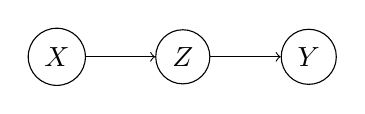
\begin{tikzpicture}[
		scale=0.8
	]

		\node[circle,draw=black] (X) at (-3,0) {$X$};
		\node[circle,draw=black] (Z) at (-1,0) {$Z$};
		\node[circle,draw=black] (Y) at (1,0) {$Y$};

		\draw[->] (X) -- (Z);
		\draw[->] (Z) -- (Y);
		
	\end{tikzpicture}
\end{figure}